\documentclass[11pt,a4paper]{article}
\usepackage[utf8]{inputenc}
\usepackage[T1]{fontenc}
\usepackage{geometry}
\usepackage{graphicx}
\usepackage{float}
\usepackage{hyperref}
\usepackage{xcolor}
\usepackage{enumitem}
\usepackage{titlesec}
\usepackage{setspace}
\usepackage{parskip}
\usepackage{fancyhdr}
\usepackage{lastpage}
\usepackage{booktabs}
\usepackage{array}
\usepackage{tabularx}
\usepackage{tcolorbox}
\usepackage{mdframed}
\usepackage{colortbl}
\usepackage{microtype}

\geometry{margin=1.25in}
\setstretch{1.15}

\definecolor{indigo}{RGB}{26,35,126}
\definecolor{indigomid}{RGB}{63,81,181}
\definecolor{indigolight}{RGB}{232,234,246}
\definecolor{amber}{RGB}{255,248,225}
\definecolor{tablealt}{RGB}{245,245,245}
\definecolor{headerbg}{RGB}{26,35,126}
\definecolor{mygray}{RGB}{85,85,85}

\hypersetup{
    colorlinks=true,
    linkcolor=indigo,
    urlcolor=indigomid,
    pdftitle={Sax Performance Booking Platform - Product Documentation},
    pdfauthor={Product Team}
}

\titleformat{\section}{\Large\bfseries\color{indigo}}{}{0em}{\vspace{0.5em}}[\vspace{0.3em}\color{indigomid}\titlerule]
\titleformat{\subsection}{\large\bfseries\color{indigo!80!black}}{}{0em}{\vspace{0.3em}}[\vspace{0.2em}]
\titleformat{\subsubsection}{\normalsize\bfseries\color{mygray}}{}{0em}{\vspace{0.2em}}

\pagestyle{fancy}
\fancyhf{}
\rhead{\small\color{indigo}\textbf{Sax Performance Booking Platform}}
\lhead{\small\color{mygray}Product Documentation}
\cfoot{\small\color{mygray}Page \thepage\ of \pageref{LastPage} \quad\textbullet\quad Confidential --- Product Team}
\renewcommand{\headrulewidth}{0.4pt}
\renewcommand{\footrulewidth}{0.4pt}

\tcbuselibrary{skins,breakable}
\newtcolorbox{callout}[2][]{
  colback=#2,
  colframe=indigomid,
  fonttitle=\bfseries,
  left=6pt, right=6pt, top=4pt, bottom=4pt,
  boxrule=0.5pt,
  #1
}

\newcolumntype{L}[1]{>{\raggedright\arraybackslash}p{#1}}

\begin{document}

% ─────────────────────────────────────────────
%  COVER PAGE
% ─────────────────────────────────────────────
\begin{titlepage}
  \centering
  \vspace*{3cm}
  {\fontsize{36}{44}\selectfont\bfseries\color{indigo} SAX PERFORMANCE\\[0.3em]
  \color{indigomid} BOOKING PLATFORM\par}
  \vspace{1em}
  {\large\color{mygray} Product Documentation \& MVP Specification\par}
  \vspace{2em}
  \textcolor{indigomid}{\rule{0.4\textwidth}{1.5pt}}
  \vspace{2em}

  \begin{tcolorbox}[colback=indigolight, colframe=indigomid, boxrule=0.5pt,
    width=0.8\textwidth, left=12pt, right=12pt, top=10pt, bottom=10pt]
    \textbf{Abstract.} This document outlines the complete product specification
    for a marketplace platform connecting event organizers with professional
    saxophone performers. It details the MVP feature set, user experience flows,
    technology architecture, and go-to-market strategy. The platform aims to
    formalize and scale the currently fragmented live sax booking ecosystem.
  \end{tcolorbox}

  \vfill
  {\normalsize\color{mygray} Product Planning \& Development Team\\[0.5em]
  \today}
\end{titlepage}

\tableofcontents
\newpage

% ─────────────────────────────────────────────
%  1. EXECUTIVE SUMMARY
% ─────────────────────────────────────────────
\section{Executive Summary}

The Sax Performance Booking Platform is a two-sided marketplace designed to
eliminate friction in booking live saxophone performers for events. By providing
structure, visibility, and trust mechanisms, the platform transforms informal
word-of-mouth referrals into a scalable, reliable talent marketplace.

\subsection*{Core Value Proposition}
\begin{itemize}[leftmargin=1.5em]
  \item \textbf{For Event Organizers:} Discover vetted performers, compare
        options, and book with confidence.
  \item \textbf{For Saxophonists:} Access consistent gig opportunities with
        transparent pricing and professional visibility.
\end{itemize}

% ─────────────────────────────────────────────
%  2. PRODUCT OVERVIEW
% ─────────────────────────────────────────────
\section{Product Overview}

\subsection{Core Concept}
The platform operates as a focused two-sided marketplace:

\begin{itemize}[leftmargin=1.5em]
  \item \textbf{Supply Side:} Saxophonists (professional, semi-professional,
        and emerging talent)
  \item \textbf{Demand Side:} Event organizers (weddings, corporate events,
        celebrations, religious ceremonies)
\end{itemize}

\textit{Market Positioning: ``The reliable, professional alternative to
informal sax booking.''}

\begin{figure}[H]
  \centering
  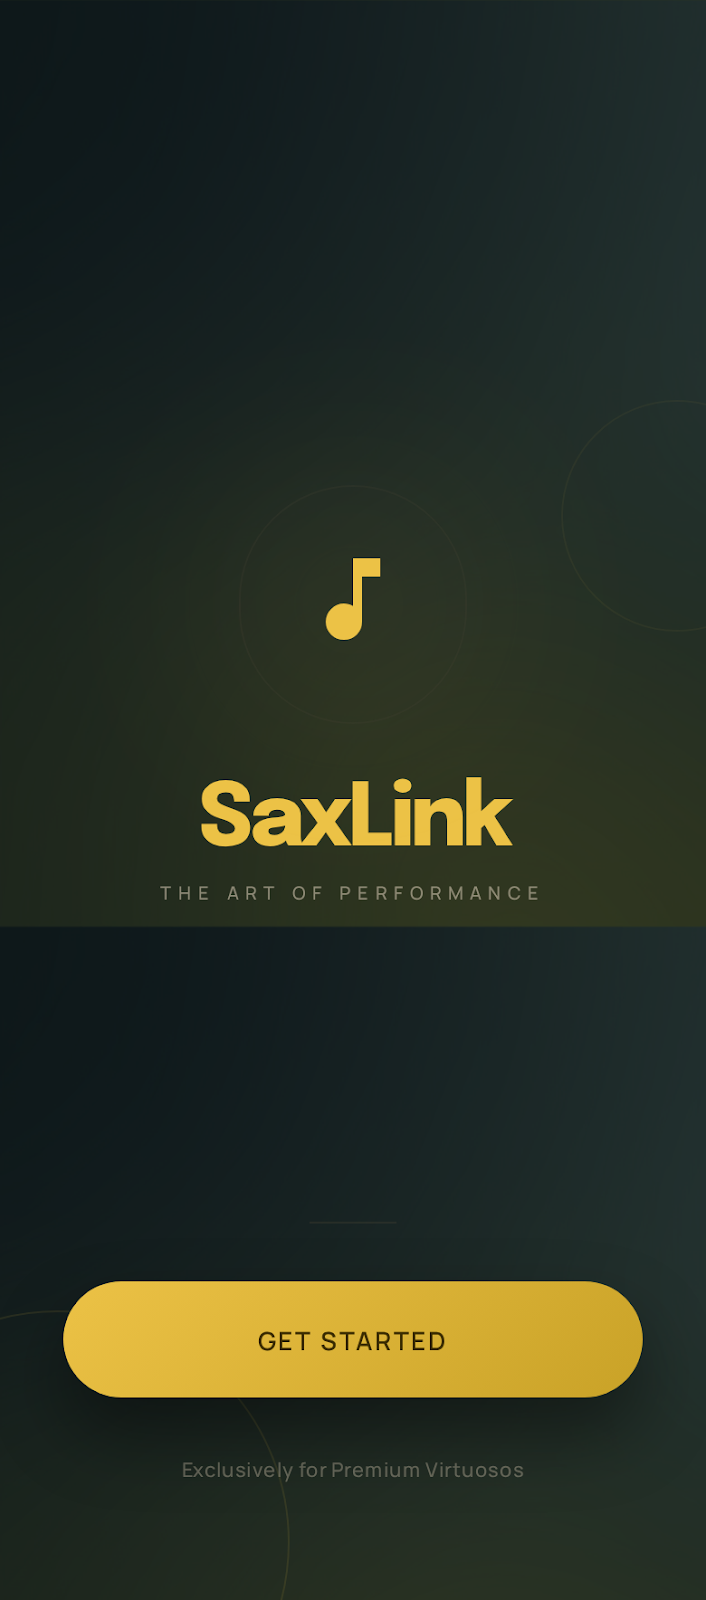
\includegraphics[width=0.32\textwidth]{splash.png}\hfill
  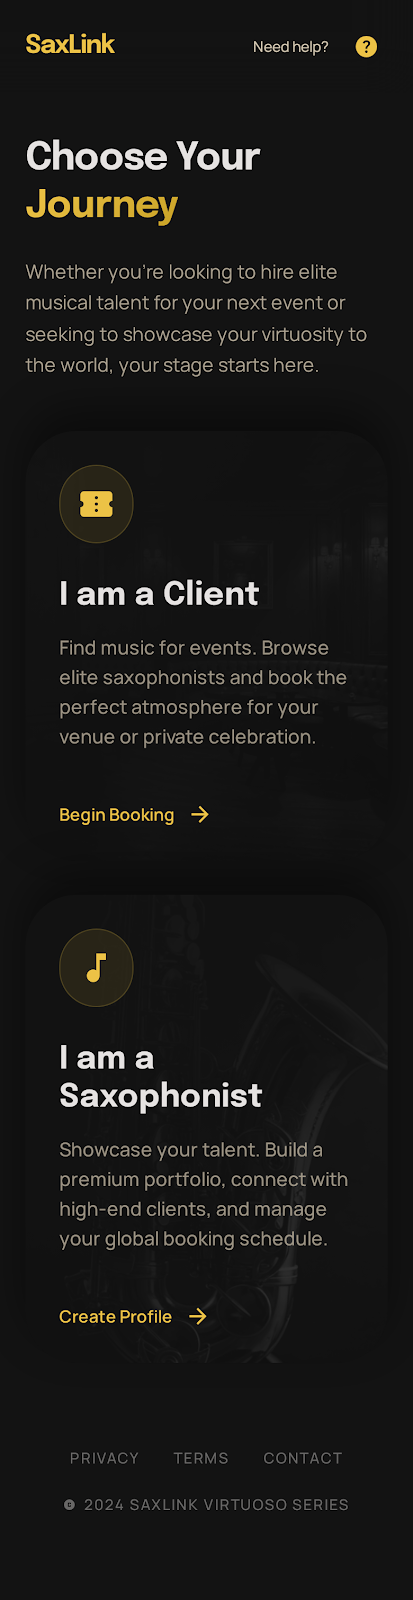
\includegraphics[width=0.32\textwidth]{role_selection.png}\hfill
  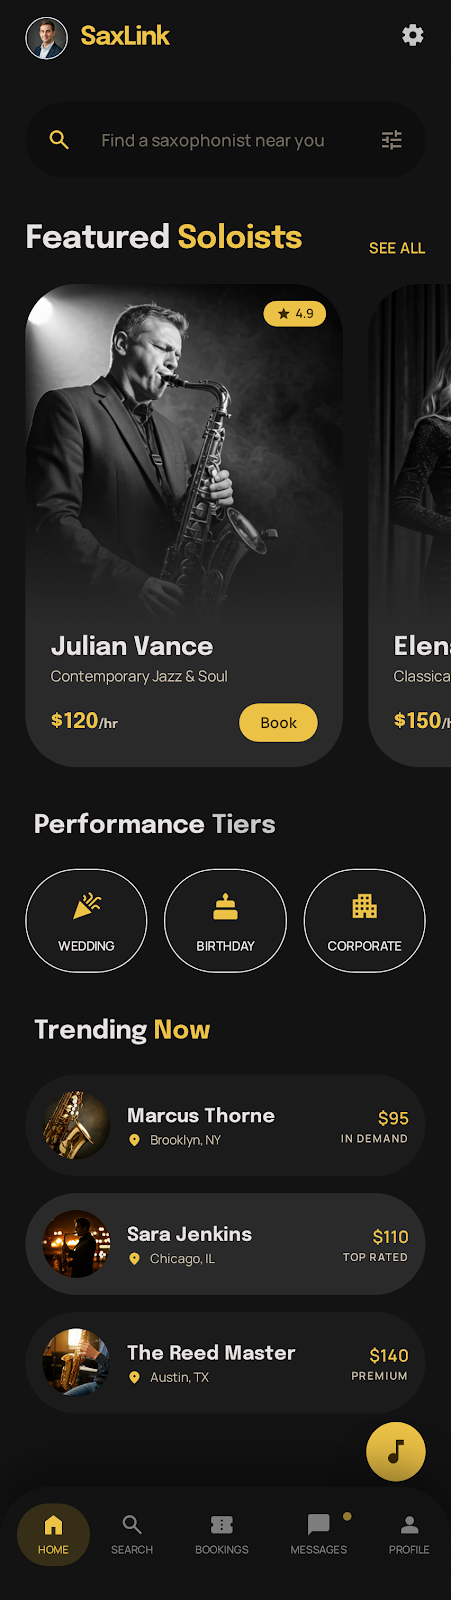
\includegraphics[width=0.32\textwidth]{client_home.png}
  \caption{Early user journey: launch, role selection, and organizer home}
\end{figure}

\subsection{Problem Statement}

\subsubsection{Current State Friction}
The existing booking ecosystem operates entirely through informal channels:
\begin{itemize}[leftmargin=1.5em]
  \item Word-of-mouth referrals with limited reach
  \item WhatsApp groups and private contact networks
  \item No standardized pricing or service definitions
  \item Last-minute cancellations and availability uncertainty
  \item No quality assurance or performance verification
  \item Difficulty for new performers to build visibility
\end{itemize}

\subsubsection{Solution Architecture}
The platform addresses these gaps through four pillars:

\begin{itemize}[leftmargin=1.5em]
  \item \textbf{Standardization:} Unified profiles, pricing models, and booking
        workflows
  \item \textbf{Discoverability:} Searchable performer database with advanced
        filtering
  \item \textbf{Trust Layer:} Ratings, reviews, verification badges, and
        performance portfolios
  \item \textbf{Operational Efficiency:} In-app messaging, automated scheduling,
        and payment processing
\end{itemize}

% ─────────────────────────────────────────────
%  3. TARGET USERS & MARKET SEGMENTS
% ─────────────────────────────────────────────
\section{Target Users \& Market Segments}

\subsection{Event Organizers (Demand Side)}

\subsubsection{Primary Segments}
\begin{itemize}[leftmargin=1.5em]
  \item \textbf{Wedding Planners:} High-budget events requiring premium talent
  \item \textbf{Corporate Event Hosts:} Team celebrations, client entertainment,
        brand activations
  \item \textbf{Religious Institutions:} Church services, ceremonies,
        celebrations
  \item \textbf{Private Party Organizers:} Birthdays, anniversaries, milestone
        celebrations
  \item \textbf{Venue Managers:} Hotels, restaurants, event spaces seeking
        entertainment partnerships
\end{itemize}

\subsubsection{User Characteristics}
\begin{itemize}[leftmargin=1.5em]
  \item Budget-conscious but quality-focused
  \item Limited network or time to source performers
  \item Require reliability and professional presentation
  \item Prefer transparent pricing and clear service terms
\end{itemize}

\subsection{Saxophonists (Supply Side)}

\subsubsection{Primary Segments}
\begin{itemize}[leftmargin=1.5em]
  \item \textbf{Professional Performers:} Full-time musicians with established
        reputations
  \item \textbf{Semi-Professional Musicians:} Part-time performers with strong
        technical skills
  \item \textbf{Emerging Talent:} Developing musicians seeking consistent
        booking opportunities
  \item \textbf{Session Musicians:} Freelancers available for short-term
        engagements
\end{itemize}

\subsubsection{User Characteristics}
\begin{itemize}[leftmargin=1.5em]
  \item Seek consistent, visible access to paid opportunities
  \item Want professional platform presence to build reputation
  \item Prefer transparent communication and fair compensation
  \item Value tools for portfolio building and audience growth
\end{itemize}

% ─────────────────────────────────────────────
%  4. MVP FEATURES
% ─────────────────────────────────────────────
\section{MVP Features (Version 1.0)}

\subsection{Saxophonist Profile System}

\subsubsection{Profile Components}
Each performer profile must include:

\begin{itemize}[leftmargin=1.5em]
  \item \textbf{Media Assets}
    \begin{itemize}[leftmargin=1.5em]
      \item High-quality profile photograph
      \item 2--5 performance videos (critical for conversion)
      \item Optional: audio clips or performance reels
    \end{itemize}
  \item \textbf{Professional Information}
    \begin{itemize}[leftmargin=1.5em]
      \item Bio (150--300 words)
      \item Musical specialties (jazz, classical, contemporary, etc.)
      \item Years of experience and notable achievements
    \end{itemize}
  \item \textbf{Operational Details}
    \begin{itemize}[leftmargin=1.5em]
      \item Primary location and service radius
      \item Hourly rate or package pricing
      \item Available dates and times
      \item Equipment provided vs.\ required
    \end{itemize}
  \item \textbf{Social Proof}
    \begin{itemize}[leftmargin=1.5em]
      \item Cumulative rating (5-star scale)
      \item Review count and recent reviews
      \item Verification badge and number of completed bookings
    \end{itemize}
\end{itemize}

\begin{callout}{amber}
  \textbf{\textcolor{indigo}{⚠\, Critical Success Factor:}} Profiles without
  performance video see 60--70\% lower conversion rates. Video content is
  non-negotiable for MVP.
\end{callout}

\begin{figure}[H]
  \centering
  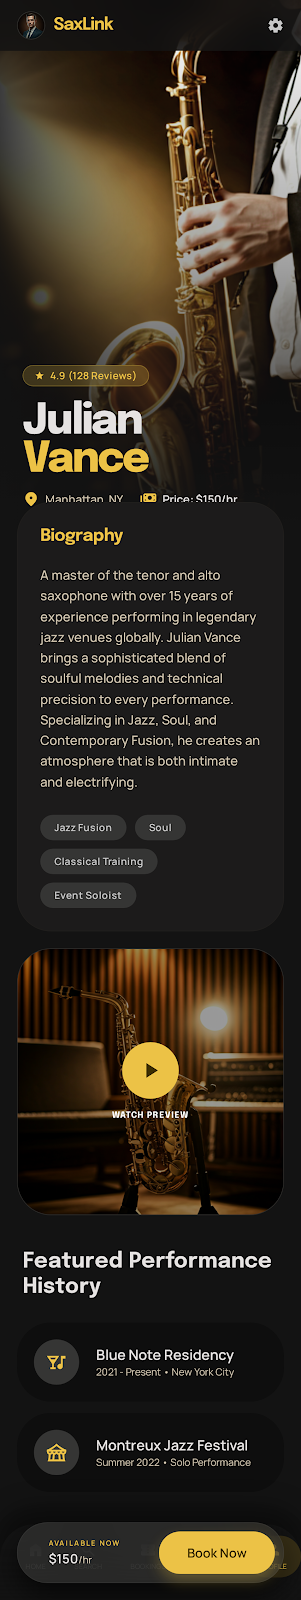
\includegraphics[width=0.42\textwidth]{profile.png}\hfill
  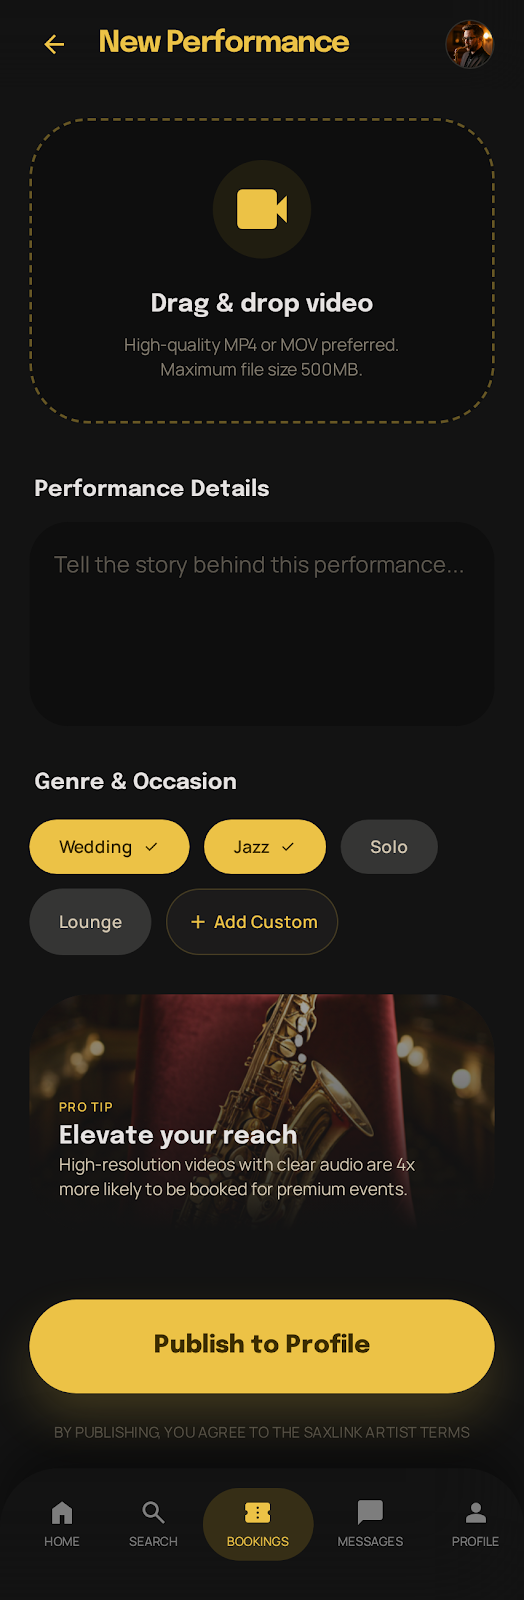
\includegraphics[width=0.42\textwidth]{performance_screen.png}
  \caption{Performer profile and performance-focused screen for trust-building}
\end{figure}

\subsubsection{Profile Creation Flow}
\begin{enumerate}[leftmargin=1.5em]
  \item Account registration (email/phone)
  \item Basic information (name, location, experience level)
  \item Profile photo upload
  \item Bio and specialties
  \item Pricing configuration
  \item Performance video upload (minimum 1 required)
  \item Availability calendar setup
  \item Profile review and publication
\end{enumerate}

\subsection{Booking System}

\subsubsection{Booking Flow Architecture}
The booking system supports two interaction modes:

\begin{itemize}[leftmargin=1.5em]
  \item \textbf{Request-Based Booking:} Organizer submits booking request;
        performer accepts or declines.
  \item \textbf{Instant Booking:} Organizer books immediately if performer has
        enabled this option.
\end{itemize}

\subsubsection{Booking Parameters}
Organizers specify the following when making a booking:

\begin{itemize}[leftmargin=1.5em]
  \item \textbf{Event Details}
    \begin{itemize}[leftmargin=1.5em]
      \item Event type (wedding, birthday, corporate, religious, other)
      \item Event date, time, and location
      \item Expected guest count
    \end{itemize}
  \item \textbf{Performance Scope}
    \begin{itemize}[leftmargin=1.5em]
      \item Duration (1 hour, 2 hours, 3+ hours, full event)
      \item Performance style preferences
      \item Specific song requests (optional)
      \item Technical requirements (sound system, staging, etc.)
    \end{itemize}
  \item \textbf{Budget \& Terms}
    \begin{itemize}[leftmargin=1.5em]
      \item Total budget or hourly rate acceptance
      \item Deposit/payment terms
      \item Cancellation policy acknowledgment
    \end{itemize}
\end{itemize}

\subsubsection{Booking Status Workflow}
\begin{enumerate}[leftmargin=1.5em]
  \item \textbf{Pending:} Organizer submits request, awaiting performer response
  \item \textbf{Confirmed:} Performer accepts, booking locked
  \item \textbf{In Progress:} Event date has arrived
  \item \textbf{Completed:} Event finished, eligible for review
  \item \textbf{Cancelled:} Either party cancels (with timestamp and reason)
\end{enumerate}

\begin{figure}[H]
  \centering
  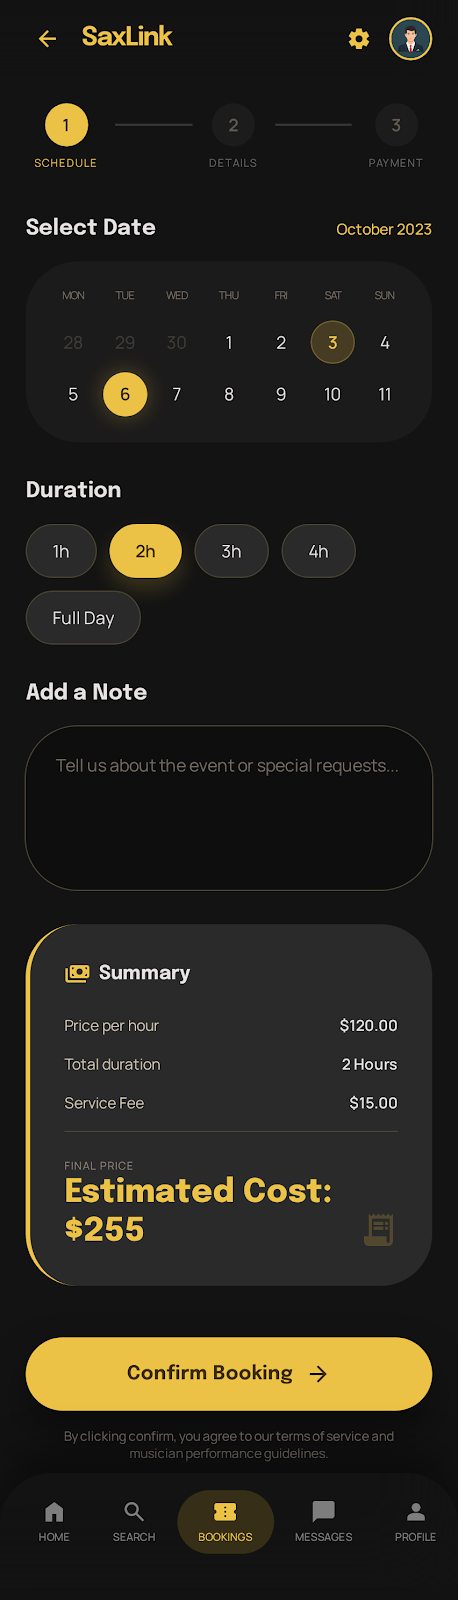
\includegraphics[width=0.70\textwidth]{booking.png}
  \caption{Booking interface aligned with request and confirmation workflows}
\end{figure}

\subsection{Discovery \& Search}

\subsubsection{Search Interface}
\begin{itemize}[leftmargin=1.5em]
  \item \textbf{Location-Based Search}
    \begin{itemize}[leftmargin=1.5em]
      \item ``Saxophonists near me'' (GPS-enabled)
      \item Manual city/area selection
      \item Service radius filtering (5\,km, 10\,km, 25\,km, etc.)
    \end{itemize}
  \item \textbf{Filter Options}
    \begin{itemize}[leftmargin=1.5em]
      \item Price range (min/max hourly rate)
      \item Rating threshold (4.5+, 4.0+, etc.)
      \item Availability (specific dates)
      \item Musical style (jazz, classical, contemporary)
      \item Experience level (emerging, professional, verified)
    \end{itemize}
  \item \textbf{Sort Options}
    \begin{itemize}[leftmargin=1.5em]
      \item Distance (nearest first)
      \item Rating (highest first)
      \item Price (lowest/highest first)
      \item Popularity (most booked) / Newest (recently joined)
    \end{itemize}
\end{itemize}

\subsubsection{Discovery Feed}
Browse mode for exploratory discovery:
\begin{itemize}[leftmargin=1.5em]
  \item Card-based performer display with photo, name, rating, and price
  \item Tap to view full profile
  \item Save/favourite performers for later comparison
\end{itemize}

\begin{figure}[H]
  \centering
  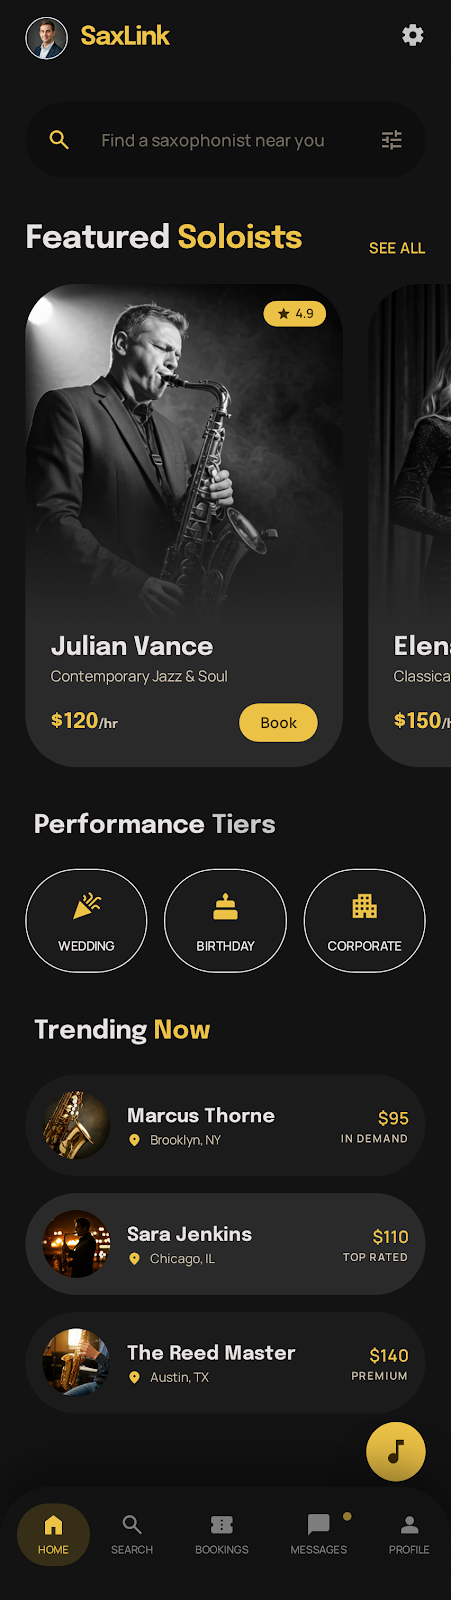
\includegraphics[width=0.70\textwidth]{client_home.png}
  \caption{Discovery view where organizers browse and compare performers}
\end{figure}

\subsection{In-App Messaging System}

\subsubsection{Messaging Features}
\begin{itemize}[leftmargin=1.5em]
  \item \textbf{Core Functionality}
    \begin{itemize}[leftmargin=1.5em]
      \item Text message exchange with full history preservation
      \item Read receipts and typing indicators
      \item Push and in-app notifications
    \end{itemize}
  \item \textbf{Contextual Features}
    \begin{itemize}[leftmargin=1.5em]
      \item Messages linked to specific booking for context
      \item Quick reply templates for common questions
      \item File/media sharing (photos, documents)
      \item Booking details accessible from chat window
    \end{itemize}
\end{itemize}

\subsubsection{Key Use Cases}
\begin{itemize}[leftmargin=1.5em]
  \item Clarify event logistics and technical requirements
  \item Negotiate scope, pricing, or special requests
  \item Share venue information and event details
  \item Build rapport and establish expectations before the event
  \item Post-event follow-up and feedback
\end{itemize}

\begin{figure}[H]
  \centering
  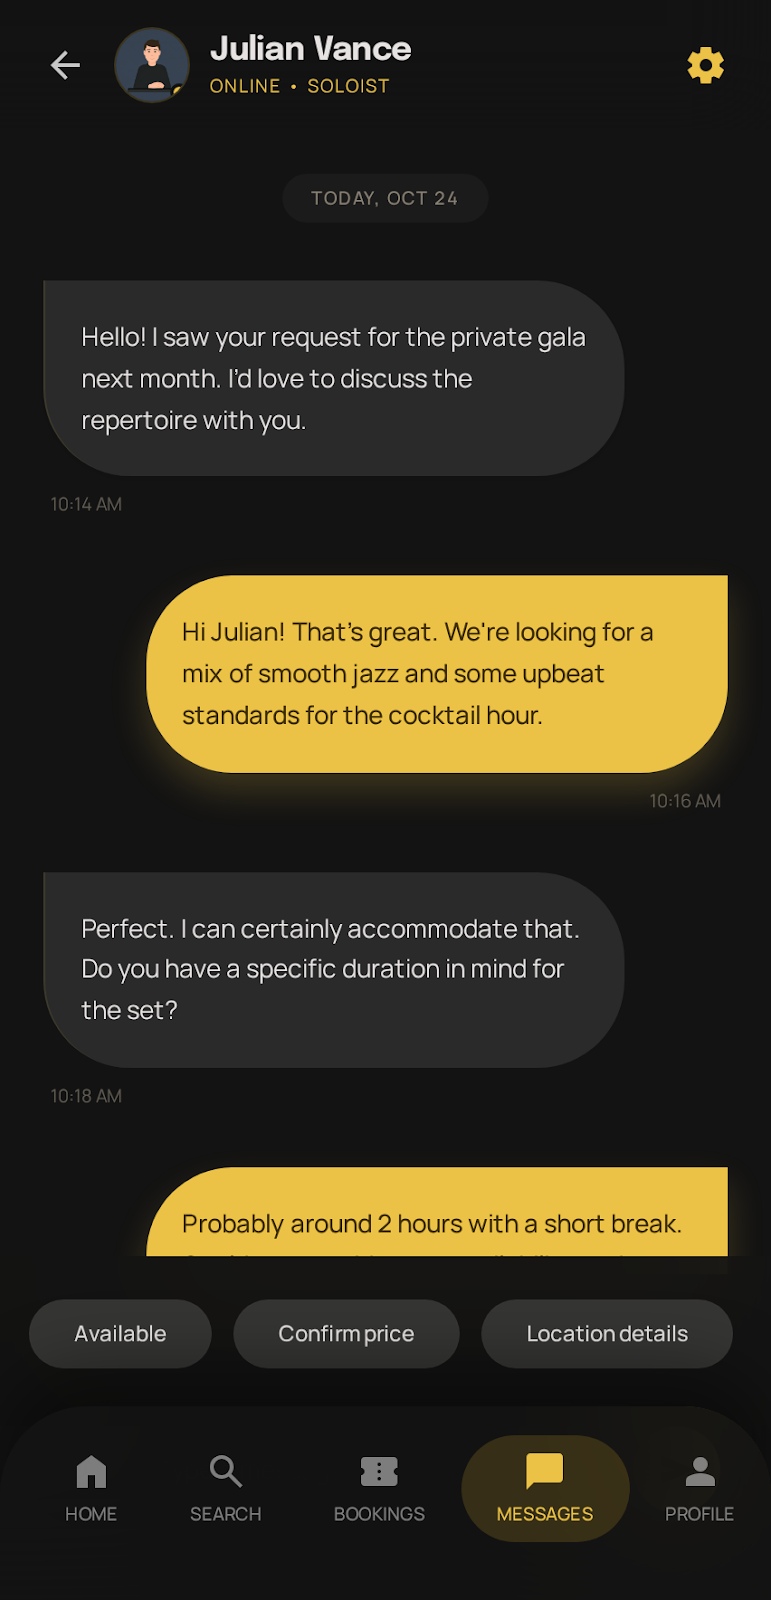
\includegraphics[width=0.52\textwidth]{chat.png}
  \caption{In-app messaging for negotiation, logistics, and confirmation}
\end{figure}

\subsection{Ratings \& Reviews System}

\subsubsection{Review Mechanics}
After event completion:
\begin{enumerate}[leftmargin=1.5em]
  \item Organizer rates performer on a 5-star scale
  \item Optional written review submitted (max 500 characters)
  \item Performer can respond publicly to any review
  \item Reviews displayed on profile (newest first)
  \item Ratings aggregated into overall performer score
\end{enumerate}

\subsubsection{Review Criteria}
Organizers evaluate performers across five dimensions:
\begin{itemize}[leftmargin=1.5em]
  \item Performance quality and musicianship
  \item Professionalism and punctuality
  \item Communication and responsiveness
  \item Value for money
  \item Overall satisfaction
\end{itemize}

\subsection{Payment System (Phase 2 Enhancement)}

\subsubsection{Payment Flow --- Future Implementation}
\begin{itemize}[leftmargin=1.5em]
  \item \textbf{Deposit System}
    \begin{itemize}[leftmargin=1.5em]
      \item Organizer pays 30--50\% deposit at booking confirmation
      \item Deposit held in escrow until event completion
      \item Released to performer post-event, or refunded if cancelled
    \end{itemize}
  \item \textbf{Full Payment}
    \begin{itemize}[leftmargin=1.5em]
      \item Remaining balance due before event date
      \item Multiple payment methods: card, mobile money, bank transfer
      \item Automated payment reminders and status tracking
    \end{itemize}
  \item \textbf{Commission Handling}
    \begin{itemize}[leftmargin=1.5em]
      \item Platform commission of 10--20\% deducted from performer payout
      \item Transparent fee breakdown shown to both parties
      \item Automated payout to performer after event completion
    \end{itemize}
\end{itemize}

\begin{callout}{indigolight}
  \textbf{\textcolor{indigo}{📌\, Note:}} MVP launches with manual payment
  coordination via in-app messaging. Integrated payments are a Phase~2
  initiative.
\end{callout}

% ─────────────────────────────────────────────
%  5. USER EXPERIENCE FLOWS
% ─────────────────────────────────────────────
\section{User Experience Flows}

\subsection{Organizer User Journey}

\subsubsection{Discovery \& Selection}
\begin{enumerate}[leftmargin=1.5em]
  \item Organizer opens app and selects ``Book a Performer'' role
  \item Searches by location, filters by date, budget, and rating
  \item Browses performer cards and views full profiles
  \item Watches performance videos and reads reviews
  \item Saves favourites for comparison
\end{enumerate}

\subsubsection{Booking \& Communication}
\begin{enumerate}[leftmargin=1.5em]
  \item Selects performer and taps ``Request Booking''
  \item Fills in event details, scope, and budget
  \item Sends booking request; receives confirmation of submission
  \item Communicates with performer via in-app messaging
  \item Receives booking confirmation when performer accepts
  \item Coordinates logistics (location, equipment, song list) via chat
\end{enumerate}

\subsubsection{Post-Event}
\begin{enumerate}[leftmargin=1.5em]
  \item Receives prompt to submit a review after event date passes
  \item Rates performer across five criteria
  \item Optionally writes a short review
  \item Review published on performer profile
\end{enumerate}

\subsection{Saxophonist User Journey}

\subsubsection{Onboarding \& Profile Setup}
\begin{enumerate}[leftmargin=1.5em]
  \item Downloads app and selects ``Performer'' role
  \item Completes guided profile setup wizard
  \item Uploads profile photo and at least one performance video
  \item Sets pricing and availability calendar
  \item Profile goes live on the platform
\end{enumerate}

\subsubsection{Managing Bookings}
\begin{enumerate}[leftmargin=1.5em]
  \item Receives push notification for new booking request
  \item Reviews event details, date, and offered terms
  \item Accepts or declines booking (with optional message)
  \item Communicates event logistics via in-app chat
  \item Marks booking as completed after event
  \item Views new review and optionally responds
\end{enumerate}

\begin{figure}[H]
  \centering
  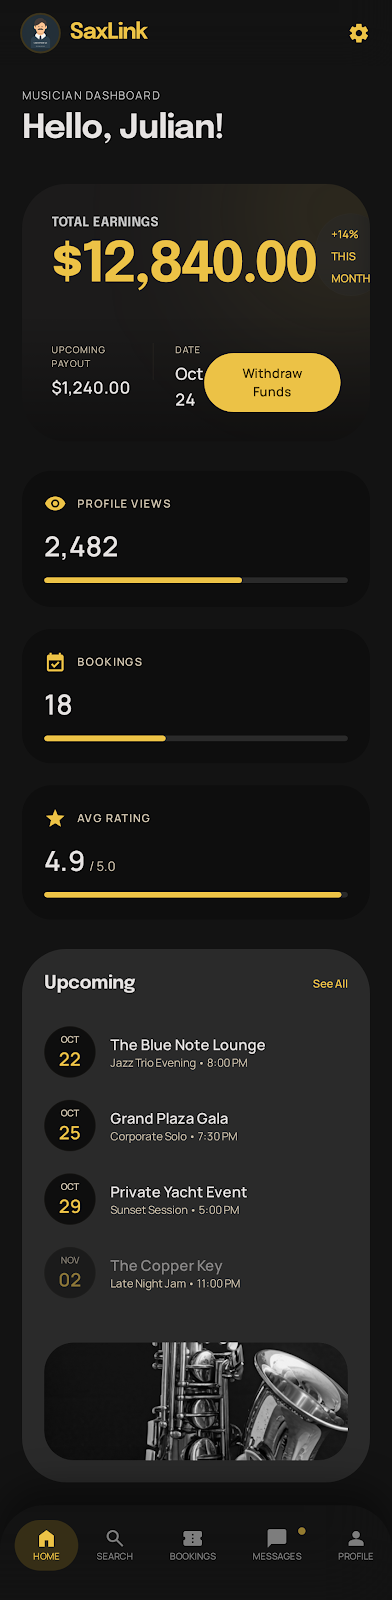
\includegraphics[width=0.60\textwidth]{dashboard.png}
  \caption{Performer dashboard for requests, activity, and booking management}
\end{figure}

% ─────────────────────────────────────────────
%  6. TECHNOLOGY ARCHITECTURE
% ─────────────────────────────────────────────
\section{Technology Architecture}

\subsection{Recommended Stack}

The following technology stack is recommended for the MVP, balancing speed of
development, scalability, and cost-effectiveness:

\vspace{0.5em}
\begin{tabularx}{\textwidth}{@{} L{3cm} L{3.5cm} X @{}}
  \toprule
  \rowcolor{headerbg}
  \textcolor{white}{\textbf{Layer}} &
  \textcolor{white}{\textbf{Technology}} &
  \textcolor{white}{\textbf{Rationale}} \\
  \midrule
  Mobile Frontend   & React Native        & Single codebase for iOS \& Android; large talent pool \\
  \rowcolor{tablealt}
  Web Frontend      & React.js            & Admin dashboard and public profile pages \\
  Backend API       & Node.js + Express   & Fast iteration; JavaScript full-stack \\
  \rowcolor{tablealt}
  Database          & PostgreSQL          & Relational data suits bookings, users, and reviews \\
  File Storage      & AWS S3 / Cloudinary & Video and image hosting with CDN delivery \\
  \rowcolor{tablealt}
  Real-Time Messaging & Socket.io         & Low-latency in-app chat \\
  Authentication    & Firebase Auth / Auth0 & Secure, managed auth with social login \\
  \rowcolor{tablealt}
  Payments (Phase 2) & Stripe / Paystack  & Africa-friendly; supports mobile money \\
  Hosting           & AWS / Railway       & Scalable infrastructure, easy deployment \\
  \bottomrule
\end{tabularx}
\vspace{0.5em}

\subsection{Key Integrations}
\begin{itemize}[leftmargin=1.5em]
  \item \textbf{Google Maps API:} Location search, radius filtering, and venue
        display
  \item \textbf{Firebase Cloud Messaging:} Push notifications for booking
        updates and messages
  \item \textbf{Cloudinary:} Optimised video/image processing and delivery
  \item \textbf{Twilio / SendGrid:} SMS and email notification fallbacks
  \item \textbf{Paystack / Stripe:} Payment processing and escrow (Phase 2)
\end{itemize}

\subsection{Security \& Compliance}
\begin{itemize}[leftmargin=1.5em]
  \item All API communication over HTTPS/TLS
  \item JWT-based authentication with refresh token rotation
  \item User data encrypted at rest (AES-256)
  \item GDPR-aligned data handling and privacy policy
  \item Media content moderation pipeline (automated + human review)
\end{itemize}

% ─────────────────────────────────────────────
%  7. GO-TO-MARKET STRATEGY
% ─────────────────────────────────────────────
\section{Go-To-Market Strategy}

\subsection{Launch Phases}

\subsubsection{Phase 1 --- Private Beta (Months 1--2)}
Invite 20--30 curated saxophonists and 10--15 event organizers to validate core
flows, surface friction points, and gather testimonials.
\begin{itemize}[leftmargin=1.5em]
  \item \textbf{Success metric:} 5+ successful bookings completed end-to-end
  \item \textbf{Focus:} Profile quality, booking flow, and messaging UX
\end{itemize}

\subsubsection{Phase 2 --- Public Launch (Months 3--4)}
Open registration with a focus on one city or region. Drive supply-side growth
first to ensure organizers find performers upon arrival.
\begin{itemize}[leftmargin=1.5em]
  \item \textbf{Target:} 50 active performer profiles in launch market
  \item \textbf{Channels:} Social media, music school partnerships, event
        planner networks
\end{itemize}

\subsubsection{Phase 3 --- Expansion (Month 5+)}
Replicate the launch playbook in additional cities/regions. Introduce referral
incentives and begin onboarding payment integrations.
\begin{itemize}[leftmargin=1.5em]
  \item \textbf{KPIs:} GMV, booking conversion rate, repeat booking rate
\end{itemize}

\subsection{Acquisition Channels}
\begin{itemize}[leftmargin=1.5em]
  \item \textbf{Saxophonists:} Direct outreach, music college partnerships,
        Facebook/Instagram musician groups
  \item \textbf{Event Organizers:} Wedding planner associations, corporate HR
        networks, venue partnerships
  \item \textbf{Content Marketing:} Blog posts on event planning tips, performer
        spotlight series
  \item \textbf{Referral Programme:} Performers earn bonus credits for every
        organizer they refer
\end{itemize}

\subsection{Revenue Model}
\begin{itemize}[leftmargin=1.5em]
  \item \textbf{Transaction Commission (Primary):} 10--20\% of each confirmed
        booking value
  \item \textbf{Featured Listings:} Performers pay to appear at the top of
        search results
  \item \textbf{Verified Badge Subscription:} Monthly fee for enhanced trust
        indicators
  \item \textbf{Premium Analytics (Future):} Performers access booking trends
        and earnings dashboards
\end{itemize}

% ─────────────────────────────────────────────
%  8. SUGGESTED IMPROVEMENTS
% ─────────────────────────────────────────────
\section{Suggested Improvements}

\subsection{Product Enhancements}
\begin{itemize}[leftmargin=1.5em]
  \item \textbf{AI-powered matching:} Surface the highest-match performers based
        on event type, budget, and organizer preferences --- reducing search
        time.
  \item \textbf{Ensemble bookings:} Extend the platform to support small bands
        and backing tracks alongside solo sax.
  \item \textbf{Recurring bookings:} Allow venues (restaurants, hotels) to set
        up weekly standing gigs with a single performer.
  \item \textbf{Pre-event checklist:} Automated reminders sent to both parties
        covering equipment, logistics, and arrival time.
  \item \textbf{Live streaming integration:} Allow performers to stream a
        mini-set as a live audition directly on their profile.
\end{itemize}

\subsection{Trust \& Safety Improvements}
\begin{itemize}[leftmargin=1.5em]
  \item \textbf{ID verification:} Require government-issued ID verification
        before a performer can accept paid bookings.
  \item \textbf{Dispute resolution:} Formal mediation workflow for cancellations
        and unfulfilled bookings.
  \item \textbf{Organizer verification:} Light KYC for organizers placing
        high-value bookings.
  \item \textbf{Background check badge:} Optional add-on for performers working
        with religious institutions or children's events.
\end{itemize}

\subsection{UX Improvements}
\begin{itemize}[leftmargin=1.5em]
  \item \textbf{Onboarding video walkthroughs:} Reduce drop-off during profile
        setup with contextual guidance.
  \item \textbf{Instant price estimator:} Organizers enter event details and get
        an estimated price range before browsing.
  \item \textbf{Calendar sync:} Two-way sync with Google Calendar / iCal for
        performers to manage availability.
  \item \textbf{Offline mode:} Cache search results and messaging history for
        low-connectivity environments.
\end{itemize}

% ─────────────────────────────────────────────
%  9. SUCCESS METRICS & KPIs
% ─────────────────────────────────────────────
\section{Success Metrics \& KPIs}

\subsection{Supply Side (Performers)}

\vspace{0.5em}
\begin{tabularx}{\textwidth}{@{} L{6cm} X @{}}
  \toprule
  \rowcolor{headerbg}
  \textcolor{white}{\textbf{Metric}} &
  \textcolor{white}{\textbf{MVP Target}} \\
  \midrule
  Performer registrations           & 50 within 60 days of launch \\
  \rowcolor{tablealt}
  Profiles with video               & $>$80\% of active profiles \\
  Average profile completion        & $>$75\% \\
  \rowcolor{tablealt}
  Performer response rate           & $>$85\% within 24 hours \\
  \bottomrule
\end{tabularx}
\vspace{0.5em}

\subsection{Demand Side (Organizers)}

\vspace{0.5em}
\begin{tabularx}{\textwidth}{@{} L{6cm} X @{}}
  \toprule
  \rowcolor{headerbg}
  \textcolor{white}{\textbf{Metric}} &
  \textcolor{white}{\textbf{MVP Target}} \\
  \midrule
  Booking requests (Month 1)        & 10+ \\
  \rowcolor{tablealt}
  Booking conversion rate           & $>$40\% \\
  Review completion rate            & $>$60\% \\
  \rowcolor{tablealt}
  Repeat booking rate (Month 3)     & $>$25\% \\
  \bottomrule
\end{tabularx}
\vspace{1em}

\vfill
\begin{center}
  \textcolor{gray}{\small\textit{--- End of Document ---}}
\end{center}

\end{document}